%----------------------------------------------------------------------------------------
%	PACKAGES AND OTHER DOCUMENT CONFIGURATIONS
%----------------------------------------------------------------------------------------

\documentclass[12pt]{article} 

\usepackage{geometry}
\geometry{a4paper} 

\usepackage{graphicx}

\usepackage{float} 
\usepackage{wrapfig} 

\usepackage{hyperref}
\usepackage{xcolor}
\hypersetup{
    colorlinks,
    linkcolor={red!50!black},
    citecolor={blue!50!black},
    urlcolor={blue!80!black}
}

%\setlength\parindent{0pt} % Uncomment to remove all indentation from paragraphs

\graphicspath{{img/}} % Specifies the directory where pictures are stored

\begin{document}

%----------------------------------------------------------------------------------------
%	TITLE PAGE
%----------------------------------------------------------------------------------------

\begin{titlepage}

\newcommand{\HRule}{\rule{\linewidth}{0.5mm}} % Defines a new command for the horizontal lines, change thickness here

\center % Center everything on the page

\textsc{\Large Hersenvulsel.be}\\[0.5cm] % Major heading such as course name
\textsc{\large Sam Gielis}\\[1cm] % Minor heading such as course title

\includegraphics[width=50mm,scale=0.5]{logo.png}\\[1cm]

\HRule \\[1cm]
{ \huge \bfseries Technische Handleiding}\\[0.8cm] % Title of your document
\HRule \\[3cm]


{\large \today}\\[3cm] % Date, change the \today to a set date if you want to be precise
\vfill % Fill the rest of the page with whitespace

\end{titlepage}

%----------------------------------------------------------------------------------------
%	TABLE OF CONTENTS
%----------------------------------------------------------------------------------------

\tableofcontents % Include a table of contents
\newpage % Begins the essay on a new page instead of on the same page as the table of contents 

%----------------------------------------------------------------------------------------
%	INTRODUCTION
%----------------------------------------------------------------------------------------

\section{Inleiding} 
Dit document is bedoeld als technische handleiding voor geverifiëerde auteurs die zelfstandig artikels op de Hersenvulsel website willen posten. Aangezien de website gehost wordt als een statische website is dit proces iets ingewikkelder dan dat het geval is bij dynamische websites, waar content gewoon via de website zelf kan toegevoegd worden.

Als auteur volg je steeds dezelfde stappen tijdens het content creatie proces. Deze inleiding geeft een kort overzicht van de te doorlopen stappen. Het proces wordt in meer detail uitgewerkt doorheen de rest van dit document.

Vooraleer je aan de slag kan als geverifiëerd Hersenvulsel auteur moet je natuurlijk eerst geverifieerd worden en enkele initiële zaken op orde brengen. Dit wordt uit de doeken gedaan in Sectie \ref{sec:init}.


\newpage






\section{Initialisatie}\label{sec:init}
Als je dit document leest betekent dat dat wij jou de kans bieden om geverifiëerd auteur te worden op Hersenvulsel. Een volwaardig deel van het team zeg maar. Als geverifiëerd auteur kan je volledig zelfstandig artikels toevoegen aan de website. Bovendien krijg je een auteursprofiel op de website dat wordt weergegeven bij de artikels die jij schrijft.

\begin{figure}[H] % Example image
\center{
\includegraphics[width=\linewidth]{auteur.png}}
\label{fig:auteur}
\end{figure}


\subsection{Een account aanmaken}
Hersenvulsel.be wordt gehost op \emph{GitHub}. Vandaar dat je zelf ook een GitHub account nodig hebt om artikels te kunnen toevoegen. Aanmelden kan \href{https://github.com/join}{hier}.

Om een Hersenvulsel account aan te maken stuur je ons een mailtje met daarin vermeld: jouw Github gebruikersnaam, een korte biografie en een persoonlijke link die geïnteresseerde lezers kunnen bezoeken. Dat kan bijvoorbeeld jouw blog zijn, een Facebook pagina of een ander account. In bijlage plaats je een foto van jezelf die minstens 280 bij 280 pixels groot is. Je kan ons contacteren op \href{mailto:schrijf@hersenvulsel.be}{schrijf@hersenvulsel.be}. Na jouw email ontvangen te hebben voegen wij jouw toe aan het Hersenvulsel project op GitHub. We maken ook een profiel aan op de Hersenvulsel website en laten iets weten wanneer dat gebeurd is.


\subsection{Git installeren}
Om artikels op de website te plaatsen moet je communcieren met de servers via \emph{git}. Dat is een systeem dat verschillende mensen aan hetzelfde project laat werken door er voor te zorgen dat verschillende files binnen het project gesycnhroniseerd blijven. 

Je kan git \href{https://git-scm.com/downloads}{hier} downloaden op de website van \emph{git-scm}. Let er tijdens de installatie zeker op dat je de command-line interface installeert. 

Wij gaan er verder vanuit dat je geen hulp nodig hebt bij de installatie. Als dat wel het geval is \href{http://hersenvulsel.be/contact/}{kan je ons altijd contacteren}.


\subsection{De Hersenvulsel website importeren}
\textcolor{red}{Let op! Deze stap kan je enkel uitvoeren als je bent toegevoegd aan het Hersenvulsel project op GitHub.}
\vspace{7 mm}

Om de website te importeren doorloop je de volgende stappen:

\begin{enumerate}
 \item{Maak een nieuwe folder aan op jouw computer waar je in wilt werken als je artikels schrijft voor Hersenvulsel. Zorg ervoor dat die folder \emph{leeg} is.}
 \item{}
\end{enumerate}






\iffalse
\subsection{Subsection 2} % Sub-section

\lipsum[2] % Dummy text

%------------------------------------------------

\subsubsection{Subsubsection 1} % Sub-sub-section

\lipsum[3] % Dummy text

\begin{figure}[H] % Example image
\center{
\includegraphics[width=0.5\linewidth]{placeholder}}
\caption{Example image.}
\label{fig:speciation}
\end{figure}

%------------------------------------------------

\subsubsection{Subsubsection 2} % Sub-sub-section

\lipsum[4] % Dummy text

%----------------------------------------------------------------------------------------
%	MAJOR SECTION 1
%----------------------------------------------------------------------------------------

\section{Content Section} % Major section

\lipsum[5] % Dummy text

%------------------------------------------------

\subsection{Subsection 1} % Sub-section

\subsubsection{Subsubsection 1} % Sub-sub-section

\lipsum[6] % Dummy text

%------------------------------------------------

\subsubsection{Subsubsection 2} % Sub-sub-section

\lipsum[6] % Dummy text
\begin{wrapfigure}{l}{0.4\textwidth} % Inline image example
  \begin{center}
    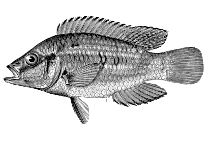
\includegraphics[width=0.38\textwidth]{fish}
  \end{center}
  \caption{Fish}
\end{wrapfigure}
\lipsum[7-8] % Dummy text

%------------------------------------------------

\subsubsection{Subsubsection 3} % Sub-sub-section

\begin{description} % Numbered list example

\item[First] \hfill \\
\lipsum[9] % Dummy text

\item[Second] \hfill \\
\lipsum[10] % Dummy text

\item[Third] \hfill \\
\lipsum[11] % Dummy text

\end{description} 

%----------------------------------------------------------------------------------------
%	MAJOR SECTION X - TEMPLATE - UNCOMMENT AND FILL IN
%----------------------------------------------------------------------------------------

%\section{Content Section}

%\subsection{Subsection 1} % Sub-section

% Content

%------------------------------------------------

%\subsection{Subsection 2} % Sub-section

% Content

%----------------------------------------------------------------------------------------
%	CONCLUSION
%----------------------------------------------------------------------------------------

\section{Conclusion} % Major section

\lipsum[12-13]

%----------------------------------------------------------------------------------------
%	BIBLIOGRAPHY
%----------------------------------------------------------------------------------------

\begin{thebibliography}{99} % Bibliography - this is intentionally simple in this template

\bibitem[Figueredo and Wolf, 2009]{Figueredo:2009dg}
Figueredo, A.~J. and Wolf, P. S.~A. (2009).
\newblock Assortative pairing and life history strategy - a cross-cultural
  study.
\newblock {\em Human Nature}, 20:317--330.
 
\end{thebibliography}
\fi
%----------------------------------------------------------------------------------------

\end{document}